
\section{Challenges and Future Directions}
\label{sec:challenges}

Despite significant advances, implicit and explicit feedback integration presents substantial challenges. This section examines current limitations and emerging research directions that will shape the next generation of recommender systems.

\begin{figure}[ht]
\centering
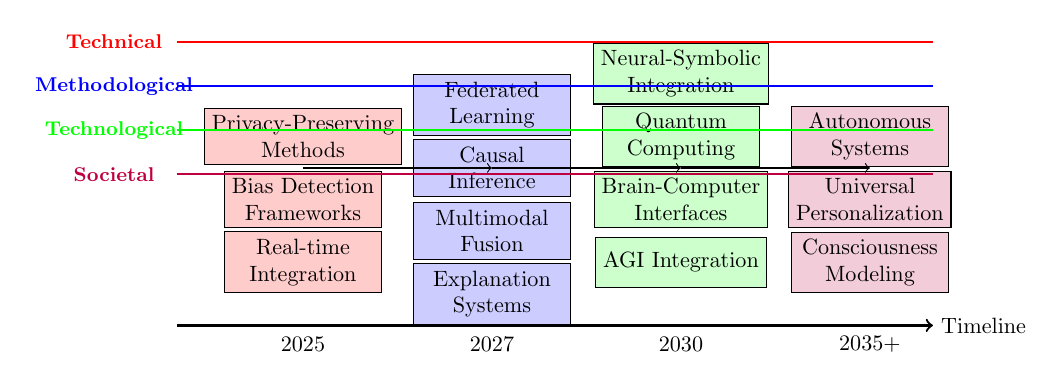
\begin{tikzpicture}[scale=0.8, transform shape]
    % Timeline
    \draw[thick, ->] (0,0) -- (12,0) node[right] {Timeline};
    \node at (2,-0.3) {2025};
    \node at (5,-0.3) {2027};
    \node at (8,-0.3) {2030};
    \node at (11,-0.3) {2035+};
    
    % Short-term (2025-2027)
    \node[rectangle, draw, fill=red!20, minimum width=2.5cm, minimum height=0.8cm, align=center] at (2,3) {Privacy-Preserving\\Methods};
    \node[rectangle, draw, fill=red!20, minimum width=2.5cm, minimum height=0.8cm, align=center] at (2,2) {Bias Detection\\Frameworks};
    \node[rectangle, draw, fill=red!20, minimum width=2.5cm, minimum height=0.8cm, align=center] at (2,1) {Real-time\\Integration};
    
    % Medium-term (2027-2030)
    \node[rectangle, draw, fill=blue!20, minimum width=2.5cm, minimum height=0.8cm, align=center] at (5,3.5) {Federated\\Learning};
    \node[rectangle, draw, fill=blue!20, minimum width=2.5cm, minimum height=0.8cm, align=center] at (5,2.5) {Causal\\Inference};
    \node[rectangle, draw, fill=blue!20, minimum width=2.5cm, minimum height=0.8cm, align=center] at (5,1.5) {Multimodal\\Fusion};
    \node[rectangle, draw, fill=blue!20, minimum width=2.5cm, minimum height=0.8cm, align=center] at (5,0.5) {Explanation\\Systems};
    
    % Long-term (2030-2035+)
    \node[rectangle, draw, fill=green!20, minimum width=2.5cm, minimum height=0.8cm, align=center] at (8,4) {Neural-Symbolic\\Integration};
    \node[rectangle, draw, fill=green!20, minimum width=2.5cm, minimum height=0.8cm, align=center] at (8,3) {Quantum\\Computing};
    \node[rectangle, draw, fill=green!20, minimum width=2.5cm, minimum height=0.8cm, align=center] at (8,2) {Brain-Computer\\Interfaces};
    \node[rectangle, draw, fill=green!20, minimum width=2.5cm, minimum height=0.8cm, align=center] at (8,1) {AGI Integration};
    
    % Future vision (2035+)
    \node[rectangle, draw, fill=purple!20, minimum width=2.5cm, minimum height=0.8cm, align=center] at (11,3) {Autonomous\\Systems};
    \node[rectangle, draw, fill=purple!20, minimum width=2.5cm, minimum height=0.8cm, align=center] at (11,2) {Universal\\Personalization};
    \node[rectangle, draw, fill=purple!20, minimum width=2.5cm, minimum height=0.8cm, align=center] at (11,1) {Consciousness\\Modeling};
    
    % Connecting arrows
    \draw[->] (2,2.5) -- (5,2.5);
    \draw[->] (5,2.5) -- (8,2.5);
    \draw[->] (8,2.5) -- (11,2.5);
    
    % Challenge categories
    \node[font=\small\bfseries] at (-1,4.5) {\textcolor{red}{Technical}};
    \node[font=\small\bfseries] at (-1,3.8) {\textcolor{blue}{Methodological}};
    \node[font=\small\bfseries] at (-1,3.1) {\textcolor{green}{Technological}};
    \node[font=\small\bfseries] at (-1,2.4) {\textcolor{purple}{Societal}};
    
    % Vertical challenge lines
    \draw[red, thick] (0,4.5) -- (12,4.5);
    \draw[blue, thick] (0,3.8) -- (12,3.8);
    \draw[green, thick] (0,3.1) -- (12,3.1);
    \draw[purple, thick] (0,2.4) -- (12,2.4);
    
\end{tikzpicture}
\caption{Research Roadmap: Future Directions for Feedback-Aware Recommender Systems}
\label{fig:research_roadmap}
\end{figure}

Figure~\ref{fig:research_roadmap} outlines the projected evolution of research challenges and opportunities across technical, methodological, technological, and societal dimensions over the next decade.

\subsection{Technical Challenges}

\subsubsection{Data Quality and Noise Issues}

Feedback signals are inherently noisy and require sophisticated processing:

\begin{itemize}
    \item \textbf{Signal Ambiguity}: Implicit feedback lacks semantic clarity, making preference interpretation challenging
    \item \textbf{Contextual Noise}: Environmental factors and user states introduce variability in feedback signals
    \item \textbf{Missing Data Patterns}: Systematic biases in feedback collection lead to incomplete preference profiles
    \item \textbf{Temporal Dynamics}: User preferences evolve over time, requiring adaptive feedback processing
    \item \textbf{Multi-device Consistency}: Feedback signals vary across platforms and devices
\end{itemize}

\subsubsection{Hybrid Integration Complexity}

Combining heterogeneous feedback types introduces algorithmic and computational challenges:

\begin{itemize}
    \item \textbf{Modal Fusion}: Developing principled approaches to combine implicit and explicit signals
    \item \textbf{Confidence Estimation}: Assessing reliability of different feedback sources
    \item \textbf{Conflict Resolution}: Handling contradictory signals from different feedback types
    \item \textbf{Feature Alignment}: Bridging semantic gaps between behavioral and declarative feedback
    \item \textbf{Scalability Trade-offs}: Balancing computational complexity with performance gains
\end{itemize}

\subsubsection{Computational and Scalability Issues}

Large-scale feedback processing demands efficient algorithms and infrastructure:

\begin{itemize}
    \item \textbf{Real-time Processing}: Handling streaming feedback at web scale
    \item \textbf{Memory Efficiency}: Managing large feedback matrices and user histories
    \item \textbf{Distributed Computing}: Coordinating feedback processing across multiple nodes
    \item \textbf{Incremental Updates}: Adapting models to new feedback without full retraining
    \item \textbf{Resource Optimization}: Balancing computational cost with recommendation quality
\end{itemize}

\subsection{Ethical and Societal Challenges}

\subsubsection{Privacy and Data Protection}

Feedback collection raises significant privacy concerns:

\begin{itemize}
    \item \textbf{Behavioral Tracking}: Continuous monitoring of user actions and patterns
    \item \textbf{Data Minimization}: Balancing feedback richness with privacy preservation
    \item \textbf{Consent Management}: Obtaining meaningful consent for feedback collection
    \item \textbf{Data Ownership}: Clarifying rights over feedback-derived insights
    \item \textbf{Regulatory Compliance}: Adhering to evolving privacy regulations (GDPR, CCPA)
\end{itemize}

\subsubsection{Bias and Fairness Considerations}

Feedback mechanisms can perpetuate or amplify societal biases:

\begin{itemize}
    \item \textbf{Selection Bias}: Non-random feedback collection leads to skewed training data
    \item \textbf{Popularity Bias}: Over-representation of popular items in feedback data
    \item \textbf{Demographic Bias}: Under-representation of certain user groups
    \item \textbf{Algorithmic Bias}: Feedback processing algorithms that disadvantage specific groups
    \item \textbf{Exposure Bias}: Limited item exposure leading to incomplete feedback landscapes
\end{itemize}

\subsubsection{User Agency and Autonomy}

Feedback collection impacts user control and decision-making:

\begin{itemize}
    \item \textbf{Transparency}: Understanding how feedback influences recommendations
    \item \textbf{Control Mechanisms}: User ability to modify or delete feedback
    \item \textbf{Manipulation Risks}: Potential for feedback manipulation by malicious actors
    \item \textbf{Filter Bubbles}: Feedback-driven personalization creating echo chambers
    \item \textbf{Decision Support}: Balancing automation with human judgment
\end{itemize}

\subsection{Evaluation and Benchmarking Challenges}

\subsubsection{Metrics and Validation}

Evaluating feedback-integrated systems requires specialized approaches:

\begin{itemize}
    \item \textbf{Offline Evaluation}: Simulating feedback characteristics in historical data
    \item \textbf{Online Evaluation}: A/B testing with real feedback collection
    \item \textbf{Cross-validation Strategies}: Accounting for feedback type dependencies
    \item \textbf{Longitudinal Assessment}: Measuring long-term system impact
    \item \textbf{User-centric Metrics}: Incorporating user satisfaction and trust measures
\end{itemize}

\subsubsection{Benchmark Datasets and Protocols}

Standardized evaluation requires appropriate data and methodologies:

\begin{itemize}
    \item \textbf{Dataset Diversity}: Representative feedback patterns across domains
    \item \textbf{Ground Truth Challenges}: Establishing reliable evaluation baselines
    \item \textbf{Reproducibility}: Ensuring consistent evaluation across research groups
    \item \textbf{Real-world Simulation}: Bridging lab and production environments
    \item \textbf{Ethical Benchmarking}: Responsible evaluation practices
\end{itemize}

\subsection{Future Research Directions}

\subsubsection{Advanced Modeling Approaches}

Emerging techniques promise to address current limitations:

\begin{itemize}
    \item \textbf{Self-supervised Learning}: Leveraging unlabeled feedback for representation learning
    \item \textbf{Multimodal Integration}: Combining textual, visual, and behavioral feedback
    \item \textbf{Graph-based Methods}: Modeling complex user-item-feedback relationships
    \item \textbf{Continual Learning}: Adapting to evolving feedback patterns
    \item \textbf{Federated Learning}: Privacy-preserving feedback processing across devices
\end{itemize}

\subsubsection{Human-Centered Design}

Future systems must prioritize user needs and values:

\begin{itemize}
    \item \textbf{Explainable Recommendations}: Providing transparent reasoning for suggestions
    \item \textbf{Interactive Feedback}: Dynamic feedback collection and refinement
    \item \textbf{Personalized Privacy}: Customizable privacy-utility trade-offs
    \item \textbf{Diverse User Support}: Accommodating different user preferences and abilities
    \item \textbf{Ethical AI Frameworks}: Integrating ethical considerations into system design
\end{itemize}

\subsubsection{Cross-Domain and Interdisciplinary Research}

Expanding the scope of feedback research:

\begin{itemize}
    \item \textbf{Cross-domain Transfer}: Applying feedback insights across application areas
    \item \textbf{Interdisciplinary Collaboration}: Integrating insights from psychology, sociology, and economics
    \item \textbf{Societal Impact Assessment}: Understanding broader implications of feedback systems
    \item \textbf{Regulatory Frameworks}: Developing appropriate governance structures
    \item \textbf{Standards Development}: Establishing industry best practices
\end{itemize}

\subsubsection{Emerging Technologies and Applications}

Emerging technologies will reshape feedback processing:

\begin{itemize}
    \item \textbf{Edge Computing}: Real-time feedback processing on user devices
    \item \textbf{Quantum Computing}: Massive-scale feedback processing for unprecedented accuracy
    \item \textbf{Brain-Computer Interfaces}: Direct neural feedback for seamless interaction
    \item \textbf{Extended Reality}: Immersive feedback collection in virtual environments
    \item \textbf{Internet of Things}: Ubiquitous feedback from connected devices
\end{itemize}

\subsection{Implementation Considerations}

\subsubsection{System Architecture}

Practical deployment requires careful architectural decisions:

\begin{itemize}
    \item \textbf{Modular Design}: Separating feedback collection, processing, and recommendation components
    \item \textbf{Real-time Pipelines}: Streaming architectures for immediate feedback processing
    \item \textbf{Scalable Storage}: Efficient management of large feedback datasets
    \item \textbf{Model Serving}: Low-latency deployment of trained recommendation models
    \item \textbf{Monitoring and Logging}: Comprehensive tracking of system performance and issues
\end{itemize}

\subsubsection{Development Best Practices}

Ensuring robust and maintainable implementations:

\begin{itemize}
    \item \textbf{Testing Frameworks}: Comprehensive validation of feedback processing pipelines
    \item \textbf{Version Control}: Managing model and data versioning for reproducible results
    \item \textbf{Continuous Integration}: Automated testing and deployment pipelines
    \item \textbf{Performance Monitoring}: Tracking system metrics and user satisfaction
    \item \textbf{Documentation}: Clear guidelines for system maintenance and extension
\end{itemize}

\subsubsection{Deployment Strategies}

Successful production deployment requires careful planning:

\begin{itemize}
    \item \textbf{Gradual Rollout}: Phased deployment with A/B testing and monitoring
    \item \textbf{User Migration}: Smooth transition from existing recommendation systems
    \item \textbf{Performance Optimization}: Tuning for production workloads and constraints
    \item \textbf{Disaster Recovery}: Backup and recovery procedures for critical components
    \item \textbf{Compliance Auditing}: Regular verification of regulatory compliance
\end{itemize}

This comprehensive analysis of challenges and future directions highlights the dynamic nature of recommendation system research, where technical, ethical, and societal considerations must be addressed in concert to advance the field toward more effective, fair, and trustworthy personalization.

\begin{itemize}
    \item \textbf{Implicit Feedback Noise}: User actions may not reflect true preferences (accidental clicks, external influences)
    \item \textbf{Explicit Feedback Bias}: Self-selection bias in rating systems, where only highly satisfied/dissatisfied users provide feedback
    \item \textbf{Contextual Interference}: Environmental factors affecting feedback interpretation (time pressure, device limitations)
    \item \textbf{Adversarial Manipulation}: Malicious users attempting to game recommendation algorithms
\end{itemize}

Mathematical formulation of noise in implicit feedback:
\begin{equation}
y_{ui} = f(p_{ui}) + \epsilon_{ui} + \eta_{ui}
\end{equation}
where $y_{ui}$ is observed feedback, $f(p_{ui})$ is true preference, $\epsilon_{ui}$ is random noise, and $\eta_{ui}$ is systematic bias.

\subsubsection{Sparsity and Cold-Start Problems}

New users and items lack sufficient feedback history:

\begin{itemize}
    \item \textbf{User Cold-Start}: New users with minimal interaction history
    \item \textbf{Item Cold-Start}: New items without feedback data
    \item \textbf{System Cold-Start}: Launching new recommendation systems from scratch
    \item \textbf{Domain Cold-Start}: Applying trained models to new domains
\end{itemize}

Hybrid approaches address sparsity through:
\begin{itemize}
    \item \textbf{Multi-Source Integration}: Combining feedback types to reduce sparsity
    \item \textbf{Transfer Learning}: Leveraging knowledge from related domains
    \item \textbf{Active Learning}: Strategically collecting feedback to maximize information gain
    \item \textbf{Zero-Shot Learning}: Making recommendations without direct feedback history
\end{itemize}

\subsubsection{Scalability and Real-Time Processing}

Large-scale systems face computational challenges:

\begin{itemize}
    \item \textbf{Data Volume}: Processing billions of feedback interactions daily
    \item \textbf{Model Complexity}: Training deep learning models on massive datasets
    \item \textbf{Real-Time Latency}: Sub-second response times for user interactions
    \item \textbf{Distributed Computing}: Coordinating feedback processing across global data centers
\end{itemize}

Optimization techniques include:
\begin{itemize}
    \item \textbf{Approximate Methods}: Using sampling and sketching for large-scale matrix factorization
    \item \textbf{Streaming Algorithms}: Online learning approaches for continuous feedback streams
    \item \textbf{Federated Learning}: Distributed training while preserving user privacy
    \item \textbf{Edge Computing}: Processing feedback closer to users for reduced latency
\end{itemize}

\subsection{Ethical and Societal Challenges}

\subsubsection{Privacy and Data Protection}

Feedback collection raises significant privacy concerns:

\begin{itemize}
    \item \textbf{Implicit Data Sensitivity}: Tracking user behavior without explicit consent
    \item \textbf{Data Minimization}: Collecting only necessary feedback while maintaining effectiveness
    \item \textbf{User Consent}: Transparent opt-in mechanisms for feedback collection
    \item \textbf{Data Ownership}: Users' rights over their feedback data
\end{itemize}

Privacy-preserving techniques:
\begin{itemize}
    \item \textbf{Differential Privacy}: Adding noise to protect individual privacy
    \item \textbf{Federated Learning}: Training models without centralizing user data
    \item \textbf{Local Differential Privacy}: Privacy protection at the device level
    \item \textbf{Homomorphic Encryption}: Computing on encrypted feedback data
\end{itemize}

\subsubsection{Fairness and Bias Mitigation}

Recommendation systems can perpetuate societal biases:

\begin{itemize}
    \item \textbf{Representation Bias}: Under-representation of minority groups in training data
    \item \textbf{Popularity Bias}: Over-recommending popular items, creating rich-get-richer effects
    \item \textbf{Position Bias}: Users' tendency to interact with highly-ranked items
    \item \textbf{Selection Bias}: Non-random feedback collection leading to skewed distributions
\end{itemize}

Fairness-aware approaches:
\begin{itemize}
    \item \textbf{Debiasing Algorithms}: Correcting for known biases in feedback data
    \item \textbf{Diverse Recommendations}: Promoting variety and serendipity
    \item \textbf{Group Fairness}: Ensuring equitable outcomes across demographic groups
    \item \textbf{Individual Fairness}: Treating similar users similarly
\end{itemize}

\subsubsection{Filter Bubbles and Echo Chambers}

Personalization can limit exposure to diverse content:

\begin{itemize}
    \item \textbf{Homophily Effects}: Users increasingly exposed to similar viewpoints
    \item \textbf{Polarization Risks}: Reinforcement of extreme opinions through feedback loops
    \item \textbf{Discovery Reduction}: Decreased exposure to novel or challenging content
    \item \textbf{Social Fragmentation}: Reduced common ground in public discourse
\end{itemize}

Mitigation strategies:
\begin{itemize}
    \item \textbf{Diversity Objectives}: Explicitly optimizing for content variety
    \item \textbf{Serendipity Injection}: Introducing unexpected but relevant recommendations
    \item \textbf{Cross-Cutting Exposure}: Balancing personalization with broad exploration
    \item \textbf{User Control}: Allowing users to adjust personalization intensity
\end{itemize}

\subsection{Explainability and Trust}

\subsubsection{Black-Box Model Transparency}

Complex models lack interpretability:

\begin{itemize}
    \item \textbf{Deep Learning Opacity}: Neural networks as uninterpretable black boxes
    \item \textbf{Hybrid Model Complexity}: Combining multiple feedback types increases opacity
    \item \textbf{Real-Time Explanations}: Providing immediate rationale for recommendations
    \item \textbf{User Comprehension}: Ensuring explanations are understandable to non-experts
\end{itemize}

Explainability techniques:
\begin{itemize}
    \item \textbf{Post-Hoc Explanations}: Interpreting model decisions after prediction
    \item \textbf{Transparent Models}: Using inherently interpretable algorithms
    \item \textbf{Local Explanations}: Explaining individual recommendations
    \item \textbf{Global Explanations}: Understanding overall model behavior
\end{itemize}

\subsubsection{User Trust and Adoption}

Building confidence in recommendation systems:

\begin{itemize}
    \item \textbf{Accuracy-Explainability Trade-off}: More accurate models often less interpretable
    \item \textbf{User Agency}: Providing control over recommendation processes
    \item \textbf{Error Recovery}: Handling and learning from incorrect recommendations
    \item \textbf{Long-term Trust}: Maintaining reliability over extended interactions
\end{itemize}

\subsection{Research Gaps and Opportunities}

\subsubsection{Theoretical Foundations}

Fundamental understanding remains incomplete:

\begin{itemize}
    \item \textbf{Feedback Theory}: Comprehensive theory of implicit vs. explicit feedback
    \item \textbf{Preference Modeling}: Mathematical models of user preference formation
    \item \textbf{Feedback Dynamics}: How feedback evolves over time and context
    \item \textbf{Causal Inference}: Understanding causal relationships in feedback loops
\end{itemize}

\subsubsection{Methodological Advances}

New approaches are needed for emerging challenges:

\begin{itemize}
    \item \textbf{Multimodal Feedback}: Integrating text, images, audio, and sensor data
    \item \textbf{Temporal Modeling}: Capturing evolving preferences over time
    \item \textbf{Social Feedback}: Leveraging social network influences
    \item \textbf{Cross-Domain Transfer}: Applying knowledge across different domains
\end{itemize}

\subsubsection{Evaluation Frameworks}

Better assessment methodologies required:

\begin{itemize}
    \item \textbf{Offline-Online Evaluation}: Bridging simulation and real-world performance
    \item \textbf{User-Centric Metrics}: Beyond accuracy to satisfaction and utility
    \item \textbf{Long-Term Effects}: Measuring sustained impact on user behavior
    \item \textbf{A/B Testing at Scale}: Rigorous experimentation in production systems
\end{itemize}

\subsection{Future Research Directions}

\subsubsection{Emerging Technologies and Paradigms}

New technologies will transform feedback utilization:

\begin{itemize}
    \item \textbf{Brain-Computer Interfaces}: Direct neural feedback for ultimate personalization
    \item \textbf{Extended Reality}: Spatial and embodied feedback in AR/VR environments
    \item \textbf{Quantum Computing}: Massive-scale optimization for recommendation problems
    \item \textbf{Edge AI}: On-device processing for privacy-preserving recommendations
\end{itemize}

\subsubsection{Interdisciplinary Integration}

Cross-disciplinary approaches will drive innovation:

\begin{itemize}
    \item \textbf{Cognitive Science}: Understanding human decision-making processes
    \item \textbf{Social Psychology}: Modeling social influence and group dynamics
    \item \textbf{Economics}: Incentive design for feedback collection and quality
    \item \textbf{Human-Computer Interaction}: Designing intuitive feedback interfaces
\end{itemize}

\subsubsection{Sustainable and Responsible AI}

Long-term societal impact considerations:

\begin{itemize}
    \item \textbf{Energy-Efficient Computing}: Reducing environmental impact of large-scale systems
    \item \textbf{Digital Well-being}: Balancing personalization with mental health
    \item \textbf{Democratic Access}: Ensuring recommendation benefits reach all societal groups
    \item \textbf{Regulatory Compliance}: Adapting to evolving privacy and fairness regulations
\end{itemize}

\subsection{Implementation Challenges}

\subsubsection{System Architecture Evolution}

Future systems will require new architectural paradigms:

\begin{itemize}
    \item \textbf{Microservices Architecture}: Modular feedback processing components
    \item \textbf{Event-Driven Systems}: Real-time feedback stream processing
    \item \textbf{Serverless Computing}: Elastic scaling for variable feedback loads
    \item \textbf{Blockchain Integration}: Decentralized feedback verification and ownership
\end{itemize}

\subsubsection{Data Infrastructure Requirements}

Supporting massive feedback volumes:

\begin{itemize}
    \item \textbf{Data Lakes}: Centralized storage for diverse feedback types
    \item \textbf{Streaming Platforms}: Real-time feedback ingestion and processing
    \item \textbf{Graph Databases}: Modeling complex user-item-feedback relationships
    \item \textbf{Vector Databases}: Efficient similarity search for high-dimensional embeddings
\end{itemize}

\subsubsection{Operational Excellence}

Production system management:

\begin{itemize}
    \item \textbf{Continuous Integration/Deployment}: Automated model updates and testing
    \item \textbf{Monitoring and Alerting}: Proactive detection of system issues
    \item \textbf{Disaster Recovery}: Ensuring system reliability and data persistence
    \item \textbf{Security Hardening}: Protecting against attacks on feedback systems
\end{itemize}

\subsection{Open Problems and Grand Challenges}

\subsubsection{Fundamental Research Questions}

Key unresolved issues:

\begin{itemize}
    \item \textbf{Feedback Sufficiency}: What is the minimum feedback required for effective recommendations?
    \item \textbf{Preference Stability}: How stable are user preferences over time and context?
    \item \textbf{Feedback Causality}: Can we establish causal links between feedback and user satisfaction?
    \item \textbf{Universal Metrics}: Are there domain-independent measures of recommendation quality?
\end{itemize}

\subsubsection{Grand Challenge Problems}

Ambitious goals for the field:

\begin{itemize}
    \item \textbf{Perfect Personalization}: Anticipating user needs before explicit expression
    \item \textbf{Universal Recommender}: Single system effective across all domains and users
    \item \textbf{Zero-Data Learning}: Making recommendations without any historical feedback
    \item \textbf{Cognitive Alignment}: Systems that understand user intent as well as humans
\end{itemize}

\subsubsection{Measurement and Benchmarking}

Establishing rigorous evaluation standards:

\begin{itemize}
    \item \textbf{Standardized Datasets}: Comprehensive benchmarks for different feedback types
    \item \textbf{Reproducibility Standards}: Ensuring research results can be independently verified
    \item \textbf{Fair Comparison}: Methodologies for comparing systems across different domains
    \item \textbf{Longitudinal Studies}: Tracking recommendation system impact over extended periods
\end{itemize}

This comprehensive analysis of challenges and future directions highlights the dynamic nature of recommendation systems research, where technical, ethical, and societal considerations must be addressed in concert to advance the field toward more effective, fair, and trustworthy personalization.
